\subsection{Studies of data from {\asas}}
\protect\label{section:asas}

{\asas} data is available over approximately a decade, although the observations
are taken less frequently than with K2. Again, flaring data obscures several of
the observations, but it was possible to find a number of periods in the data
during which little or no flaring took place. In Fig. \ref{fig:asaslcurve} is
shown one such period and the light curve. A periodogram was produced from this,
showing a peak at 2.87 days as shown in Fig. \ref{fig:asaspgram}.

\begin{figure}[!htbp]
\begin{center}
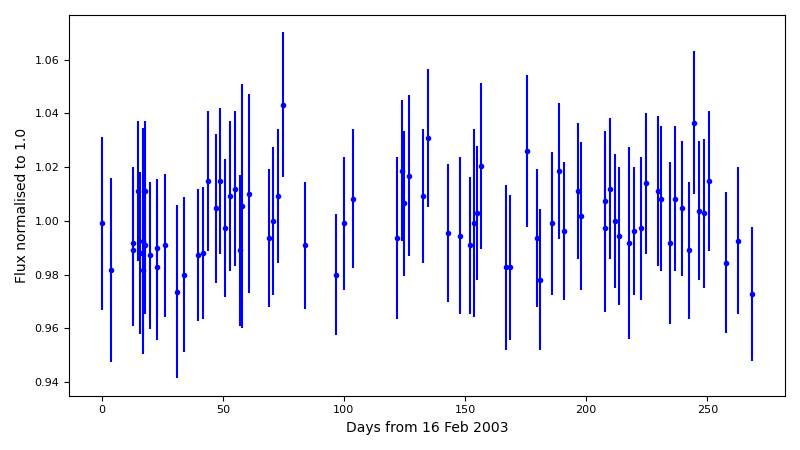
\includegraphics[scale=0.40]{asas/images/asaslcurve.png} \\
\vspace{-.5cm}
\end{center}   
\caption{Data for {\ross} taken from the {\asas} archive for nearly a year from
January 2003 onward, selecting only Class A and
B data. This display shows the reported error bar
for each observation, the reported magnitude
value being shown as a single point.}\protect\label{fig:asaslcurve}
\end{figure}

\begin{figure}[!htbp]
\begin{center}
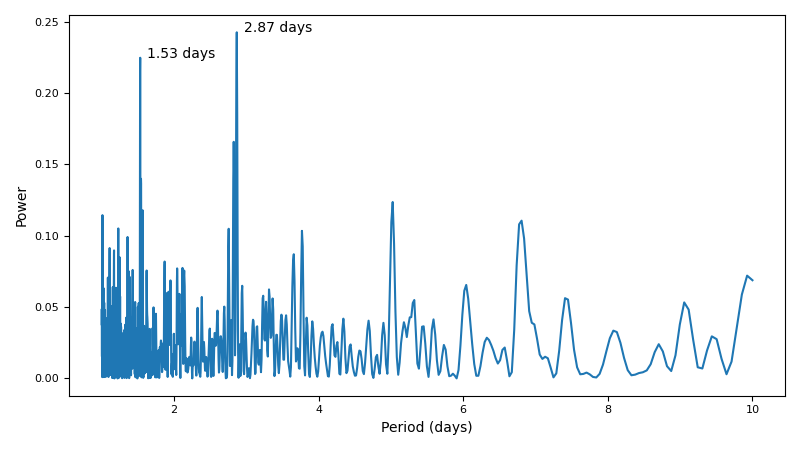
\includegraphics[scale=0.40]{asas/images/asaspgram.png} \\
\vspace{-.5cm}
\end{center}   
\caption{Periodogram taken from the data displayed in Fig.
\ref{fig:asaslcurve}.}\protect\label{fig:asaspgram}
\end{figure}

